% Meetings: four meetings that went wrong, and what the class makes of them.
% Shared preamble for the write-on class slides.
%
% Every deck is designed to be projected and annotated live on a tablet:
% whatever takes time to draw is pre-drawn, and whatever the class produces is
% left blank. Compile a deck with `pdflatex main.tex` from its own directory,
% or run `uv run python build.py` from the repository root to build them all.
\documentclass[10pt]{article}

\usepackage[papersize={25.6cm,14.4cm}, margin=1.1cm, bottom=1.5cm,
            footskip=0.75cm]{geometry}
\usepackage[T1]{fontenc}
\usepackage[default]{sourcesanspro}
\usepackage{newtxsf}
\usepackage{tikz}
\usepackage{amsmath}
\usepackage{parskip}
\usepackage{fancyhdr}
\usetikzlibrary{arrows.meta, positioning, calc}

\setlength{\parindent}{0pt}

% Catppuccin Latte, the palette the course site uses in its light theme, so a
% deck on the projector looks like the pages the students read.
\definecolor{inkbg}{HTML}{EFF1F5}      % base
\definecolor{inksurface}{HTML}{E6E9EF} % mantle
\definecolor{inkfaint}{HTML}{CCD0DA}   % surface2, for rules and empty boxes
\definecolor{inktext}{HTML}{4C4F69}    % text
\definecolor{inkgrey}{HTML}{8C8FA1}    % overlay1, for anything secondary
\definecolor{inkblue}{HTML}{7287FD}    % lavender, the primary accent
\definecolor{inkteal}{HTML}{179299}    % teal
\definecolor{inkred}{HTML}{FE640B}     % peach, for whatever wants attention
\definecolor{inkmauve}{HTML}{8839EF}   % mauve

\pagecolor{inkbg}
\color{inktext}

% A box to write a short answer into. White against the tinted page, so it
% reads as somewhere to write rather than as part of the printed material.
\newcommand{\blank}[1][1.6]{%
  \tikz[baseline=(current bounding box.base)]{%
    \draw[inkfaint, line width=0.7pt, rounded corners=2pt, fill=white]
      (0,-0.18) rectangle (#1,0.62);}}

% A ruled area to work in. Faint dots keep handwriting level on a tablet.
\newcommand{\workspace}[2]{%
  \begin{tikzpicture}
    \draw[inkfaint, line width=0.7pt, rounded corners=3pt, fill=white]
      (0,0) rectangle (#1,#2);
    \foreach \gx in {0.5,1.0,...,#1}{%
      \foreach \gy in {0.5,1.0,...,#2}{%
        \fill[inkfaint] (\gx,\gy) circle (0.5pt);}}
  \end{tikzpicture}}

% A panel for material that is printed rather than written on.
\newcommand{\panel}[2]{%
  \begin{tikzpicture}
    \draw[inkfaint, line width=0.7pt, rounded corners=3pt, fill=inksurface]
      (0,0) rectangle (#1,#2);
  \end{tikzpicture}}

% A labelled card of printed material. #2 and #3 are widths in cm; the text
% column is the card less its padding, computed rather than guessed.
\newcommand{\cardbox}[4]{%
  \begin{tikzpicture}
    \node[draw=#1, line width=1pt, rounded corners=4pt, fill=white,
          minimum width=#2cm, minimum height=#3cm,
          text width=\dimexpr#2cm-0.9cm\relax,
          align=left, inner sep=0.45cm, text=inktext] {#4};
  \end{tikzpicture}}

% A card whose body is left blank for the class to fill in.
\newcommand{\cardblank}[4]{%
  \begin{tikzpicture}
    \node[draw=#1, line width=1pt, rounded corners=4pt, fill=white,
          minimum width=#2cm, minimum height=#3cm,
          text width=\dimexpr#2cm-0.9cm\relax,
          align=left, inner sep=0.45cm, text=inktext, anchor=north west]
      at (0,0) {#4};
  \end{tikzpicture}}

% Running header: the deck name on the left, the page's own step on the right.
% Each deck sets its name once with \deckname.
\newcommand{\deck}{}
\newcommand{\deckname}[1]{\renewcommand{\deck}{#1}}
\newcommand{\slidehead}[1]{%
  {\small\color{inkgrey}%
   \tikz[baseline=-0.5ex]{\fill[inkblue, rounded corners=1pt]
     (0,0) rectangle (0.22,0.22);}\;\deck
   \hfill \color{inkblue}\bfseries #1}\par
  {\color{inkblue}\rule{\linewidth}{1pt}}\par\vspace{0.35em}}

\pagestyle{fancy}
\fancyhf{}
\renewcommand{\headrulewidth}{0pt}
\fancyfoot[R]{\small\color{inkgrey}\thepage}

% Deck title pages, which carry no header and no page number.
\newcommand{\titleslide}[3]{%
  \thispagestyle{empty}%
  \begin{center}
    \vspace*{\fill}
    {\Huge\bfseries\color{inkblue} #1}\\[0.7em]
    {\LARGE\color{inkgrey} #2}\\[2.4em]
    #3
    \vspace*{\fill}
  \end{center}}

% One step of the plan on a title page.
\newcommand{\stepbox}[3]{%
  \node[draw=inkblue, line width=0.9pt, rounded corners=4pt, fill=white,
        minimum width=6cm, minimum height=1.7cm, align=center,
        text=inktext] (#1) at (#2,0) {#3};}

% Prompt to the room: a question the class answers, not something I read out.
\newcommand{\ask}[1]{%
  {\large\color{inkblue}\bfseries #1}\par\vspace{0.5em}}


\deckname{Meetings}

\begin{document}

\titleslide{Meetings}{Four meetings that went wrong}{%
    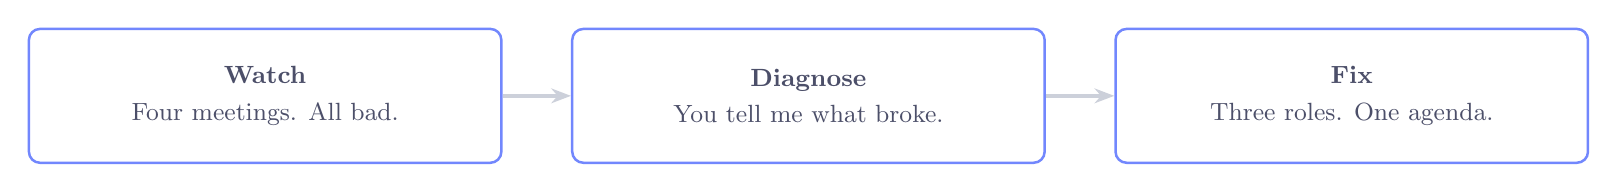
\begin{tikzpicture}[font=\small]
      \stepbox{s0}{0.0}{\textbf{Watch}\\[0.25em] Four meetings. All bad.}
      \stepbox{s1}{6.9}{\textbf{Diagnose}\\[0.25em] You tell me what broke.}
      \stepbox{s2}{13.8}{\textbf{Fix}\\[0.25em] Three roles. One agenda.}
      \draw[-{Stealth[length=2.5mm]}, inkfaint, line width=1.2pt] (s0) -- (s1);
      \draw[-{Stealth[length=2.5mm]}, inkfaint, line width=1.2pt] (s1) -- (s2);
    \end{tikzpicture}}

\newpage
\slidehead{A meeting is not a workshop}

\vspace{0.5cm}

\begin{center}

\begin{tikzpicture}
  \node at (0,0) {\cardbox{inkteal}{9.6}{3.0}{%
    {\large\bfseries\color{inkteal} Meeting}\\[0.5em]
    {\large Agenda. Turns. Decisions.}}};
  \node at (12.2,0) {\cardbox{inkblue}{9.6}{3.0}{%
    {\large\bfseries\color{inkblue} Workshop}\\[0.5em]
    {\large No agenda. Laptops. Work.}}};
  \draw[-{Stealth[length=3mm]}, inkfaint, line width=1.4pt]
    (5.1,0) -- (7.4,0) node[midway, above, font=\small, text=inkgrey] {then};
\end{tikzpicture}
\end{center}

\vspace{0.5cm}

\ask{Which one have your group sessions been so far?}

\newpage
\slidehead{Every agenda item is one of three}

\vspace{0.8cm}

\begin{center}

\begin{tikzpicture}
  \node at (0,0) {\cardbox{inkblue}{6.4}{2.2}{%
    {\large\bfseries\color{inkblue} Inform}}};
  \node at (7.3,0) {\cardbox{inkteal}{6.4}{2.2}{%
    {\large\bfseries\color{inkteal} Discuss}}};
  \node at (14.6,0) {\cardbox{inkred}{6.4}{2.2}{%
    {\large\bfseries\color{inkred} Decide}}};
\end{tikzpicture}
\end{center}

\vspace{0.9cm}

\begin{center}
{\LARGE If you cannot say which one an item is, it is not ready.}
\end{center}

\newpage
\slidehead{1. No agenda}

\vspace{0.4cm}

\begin{center}
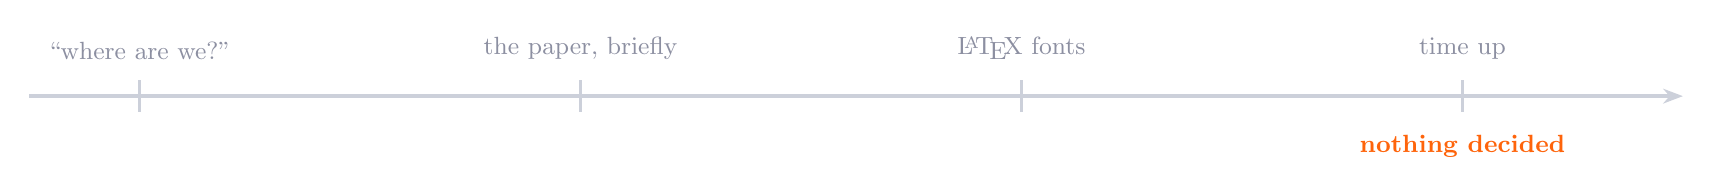
\begin{tikzpicture}[scale=1.0]
  \draw[-{Stealth[length=2.5mm]}, inkfaint, line width=1.2pt] (0,0) -- (21,0);
  \foreach \x/\lbl in {
    1.4/{``where are we?''}, 7.0/{the paper, briefly},
    12.6/{\LaTeX{} fonts}, 18.2/{time up}}
    {\draw[inkfaint, line width=1pt] (\x,0.2) -- (\x,-0.2);
     \node[font=\small, text=inkgrey, align=center, above=4pt] at (\x,0.2)
       {\lbl};}
  \node[font=\small\bfseries, text=inkred, below=5pt] at (18.2,-0.2)
    {nothing decided};
\end{tikzpicture}
\end{center}

\vspace{0.5cm}

\ask{What does the secretary write in the minutes?}

\begin{center}
\workspace{22}{4.6}
\end{center}

\newpage
\slidehead{2. A workshop in disguise}

\vspace{0.3cm}

\begin{minipage}[t]{0.46\linewidth}
\vspace{0pt}
{\large
\textbf{10:00} Item 1: report on Chapter 3.\\[0.45em]
\textbf{10:04} B spots a bug. Everyone leans in.\\[0.45em]
\textbf{10:40} Bug fixed. A good fix.\\[0.45em]
\textcolor{inkred}{\textbf{10:41} Items 2, 3, 4 never reached.}\\[0.45em]
\textcolor{inkred}{\textbf{10:42} D, silent throughout, leaves.}}
\end{minipage}
\hfill
\begin{minipage}[t]{0.50\linewidth}
\vspace{0pt}
\ask{Real work got done. What did it cost D?}

\workspace{11.4}{5.4}
\end{minipage}

\newpage
\slidehead{3. One person ran it}

\vspace{0.2cm}

\begin{minipage}[t]{0.44\linewidth}
\vspace{0pt}
\begin{center}
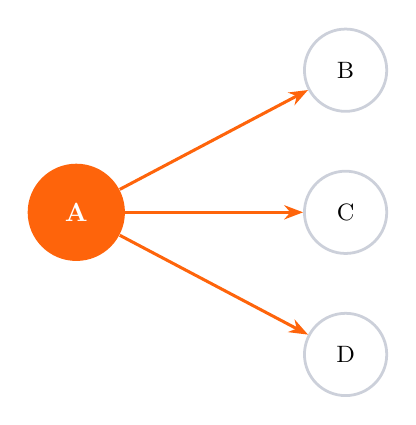
\begin{tikzpicture}[scale=0.95, every node/.style={transform shape}]
  \node[circle, fill=inkred, text=white, minimum size=1.3cm,
        font=\bfseries] (a) at (0,0) {A};
  \foreach \n/\y in {B/1.9, C/0, D/-1.9}{%
    \node[circle, draw=inkfaint, line width=1pt, fill=white,
          minimum size=1.1cm, font=\small] (\n) at (3.6,\y) {\n};
    \draw[-{Stealth[length=2.4mm]}, inkred, line width=1.1pt] (a) -- (\n);}
\end{tikzpicture}
\end{center}

\vspace{0.3em}

{\large\color{inkgrey} 35 of 40 minutes. Everyone agreed.\\
Minutes: three decisions, no disagreement.}
\end{minipage}
\hfill
\begin{minipage}[t]{0.52\linewidth}
\vspace{0pt}
\ask{The minutes look perfect. What is missing?}

\workspace{11.8}{5.8}
\end{minipage}

\newpage
\slidehead{4. No record}

\vspace{0.4cm}

\begin{center}

\begin{tikzpicture}
  \node at (0,0) {\cardbox{inkteal}{9.0}{3.0}{%
    {\large\bfseries\color{inkteal} In the room}\\[0.4em]
    {\large Good discussion. A real decision.}}};
  \node at (12.0,0) {\cardbox{inkred}{9.0}{3.0}{%
    {\large\bfseries\color{inkred} A week later}\\[0.4em]
    {\large Who agreed what? No minutes.}}};
  \draw[-{Stealth[length=3mm]}, inkfaint, line width=1.4pt]
    (4.8,0) -- (7.2,0);
\end{tikzpicture}
\end{center}

\ask{Nothing went wrong in the room. What did it cost?}

\begin{center}
\workspace{22}{3.2}
\end{center}

\newpage
\slidehead{So what fixes all four?}

\vspace{0.5cm}

\begin{center}
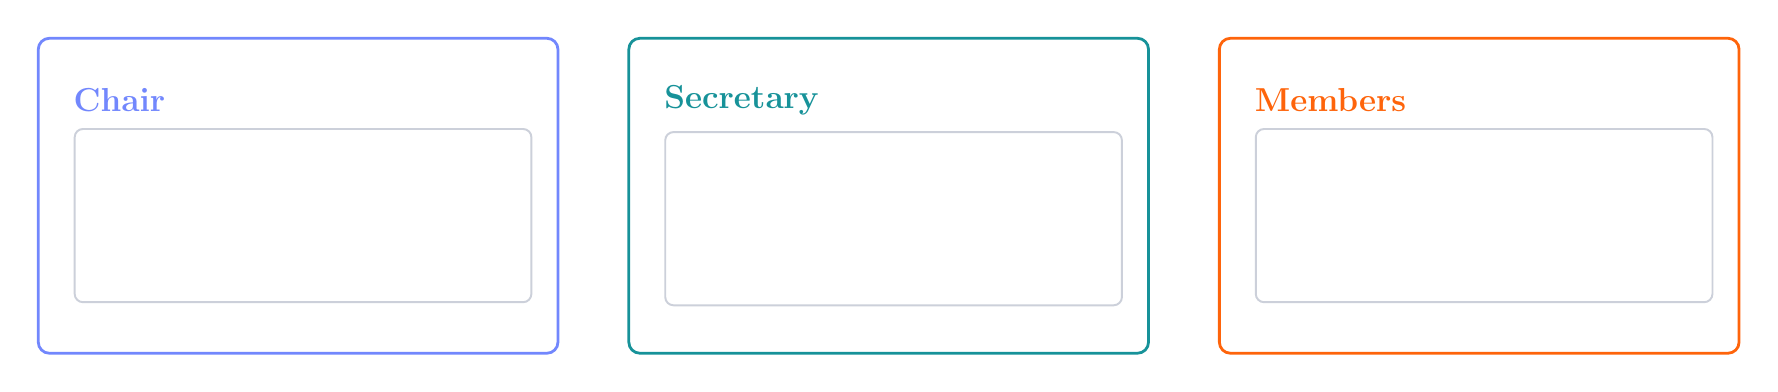
\begin{tikzpicture}
  \node at (0,0) {\cardbox{inkblue}{6.6}{4.0}{%
    {\large\bfseries\color{inkblue} Chair}\\[0.5em]
    \tikz{\draw[inkfaint, line width=0.7pt, rounded corners=3pt, fill=white]
      (0,0) rectangle (5.8,2.2);}}};
  \node at (7.5,0) {\cardbox{inkteal}{6.6}{4.0}{%
    {\large\bfseries\color{inkteal} Secretary}\\[0.5em]
    \tikz{\draw[inkfaint, line width=0.7pt, rounded corners=3pt, fill=white]
      (0,0) rectangle (5.8,2.2);}}};
  \node at (15.0,0) {\cardbox{inkred}{6.6}{4.0}{%
    {\large\bfseries\color{inkred} Members}\\[0.5em]
    \tikz{\draw[inkfaint, line width=0.7pt, rounded corners=3pt, fill=white]
      (0,0) rectangle (5.8,2.2);}}};
\end{tikzpicture}
\end{center}

\vspace{0.5cm}

\ask{What does each of them actually do? And how often do they change?}

\newpage
\slidehead{Your standing agenda}

\vspace{1.2cm}

{\LARGE
\textbf{\color{inkblue}1. Inform.}\quad What each member read.

\vspace{1.1em}

\textbf{\color{inkteal}2. Discuss.}\quad Questions, and the project.

\vspace{1.1em}

\textbf{\color{inkred}3. Decide.}\quad Who does what, by when.}

\vspace{1.3cm}

{\large\color{inkgrey} Every week. The secretary writes it down as you go.}

\newpage
\slidehead{This is how \(I\) is measured}

\vspace{0.8cm}

\begin{center}
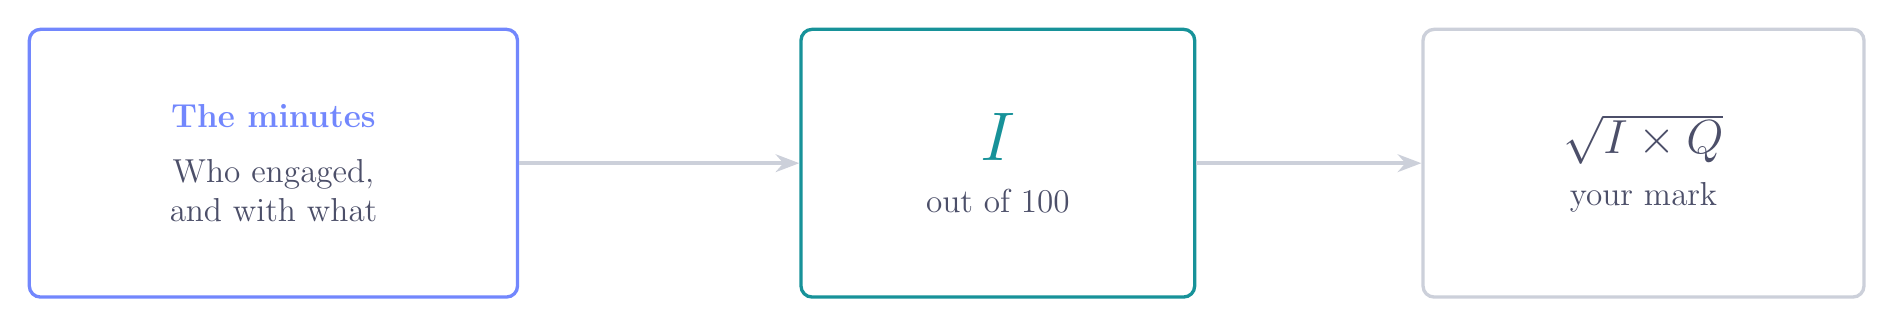
\begin{tikzpicture}
  \node[draw=inkblue, line width=1.2pt, rounded corners=4pt, fill=white,
        minimum width=6.2cm, minimum height=3.4cm, align=center,
        font=\large, text=inktext] (form)
    {\textbf{\color{inkblue} The minutes}\\[0.5em] Who engaged,\\ and with what};
  \node[draw=inkteal, line width=1.2pt, rounded corners=4pt, fill=white,
        minimum width=5.0cm, minimum height=3.4cm, align=center,
        font=\large, text=inktext] (i) at (9.2,0)
    {{\Huge\bfseries\color{inkteal} \(I\)}\\[0.4em] out of 100};
  \node[draw=inkfaint, line width=1.2pt, rounded corners=4pt, fill=white,
        minimum width=5.6cm, minimum height=3.4cm, align=center,
        font=\large, text=inktext] (mark) at (17.4,0)
    {{\LARGE \(\sqrt{I \times Q}\)}\\[0.4em] your mark};
  \draw[-{Stealth[length=3mm]}, inkfaint, line width=1.4pt] (form) -- (i);
  \draw[-{Stealth[length=3mm]}, inkfaint, line width=1.4pt] (i) -- (mark);
\end{tikzpicture}
\end{center}

\vspace{0.9cm}

\begin{center}
{\LARGE Meet \textbf{this week} in your own group slot.\\[0.4em]
 Bring the completed Week 4 minutes to \textbf{the next session}.}
\end{center}

\vspace{0.5em}

\begin{center}
{\large\color{inkgrey} No minutes handed in means no record of
engagement, for every member of the group.}
\end{center}

\newpage
\slidehead{Before you leave}

\vspace{0.7cm}

{\LARGE
\textbf{\color{inkblue}1.}\quad Agree your \textbf{secretary rota}:
\blank[3]\ \blank[3]\ \blank[3]\ \blank[3]

\vspace{1.0em}

\textbf{\color{inkblue}2.}\quad Agree \textbf{when and where} you meet:
\blank[7]

\vspace{1.0em}

\textbf{\color{inkblue}3.}\quad Next week's chair: \blank[5]

\vspace{1.0em}

\textbf{\color{inkred}4.}\quad \textbf{Meet this week. Bring the
minutes to the next session.}}

\socialfooter

\end{document}
